% ============================================================
%   main.tex —— 深圳大学实验报告（主文件）
% ============================================================

\documentclass[12pt, a4paper]{article}
\usepackage{szu_lab}

\begin{document}

% ============================================================
%   第一页：封面
% ============================================================
\newgeometry{top=3cm, bottom=3cm, left=3.5cm, right=2.5cm}

\begin{center}
    \vspace*{0.5cm}
    {\fontsize{26pt}{30pt}\selectfont\bfseries 深\enspace 圳\enspace 大\enspace 学\enspace 实\enspace 验\enspace 报\enspace 告}
    \vspace{2cm}
\end{center}

\newcommand{\mline}[2]{%
    \noindent\mbox{\zihao{4}\bfseries #1：\underline{\makebox[10cm][l]{#2}}}\\[3ex]%
}

\vspace{0.5cm}
\begin{flushleft}
    \mline{课程名称}{人工智能}
    \mline{实验项目名称}{基于 YOLOv11 的行人和车辆检测}
    \mline{学\hspace{2em}院}{电子与信息工程学院}
    \mline{专\hspace{2em}业}{电子与信息工程}
    \mline{指导教师}{戴林蕙}
    \noindent\mbox{\zihao{4}\bfseries
        报告人：\underline{\makebox[3cm][l]{戴西西(cat)}}%
        \hspace{1.5em}学号：\underline{\makebox[3.5cm][l]{20240615}}%
        \hspace{1.5em}班级：\underline{\makebox[3cm][l]{电信2401}}%
    }\\[3ex]
    \mline{实验时间}{2026 年 3 月 23 日}
    \mline{实验报告提交时间}{2026 年 4 月 1 日}
\end{flushleft}

\vfill
\begin{center}
    {\large \textbf{教\enspace 务\enspace 部\enspace 制}}
\end{center}

\newpage
\restoregeometry


% ============================================================
%   一、实验目的与要求
% ============================================================
\begin{labbox}{一、实验目的与要求：}{}

\begin{itemize}[leftmargin=2em, itemsep=0.3em]
    \item 了解 YOLO 系列目标检测算法的发展历程，掌握 YOLOv11 的网络结构与核心改进。
    \item 学习在 Anaconda 中创建独立虚拟环境，并完成 Ultralytics 框架的安装与配置。
    \item 掌握通过 Roboflow 获取小规模标注数据集的方法，无需手工标注即可完成数据准备。
    \item 能够在 CPU 环境下对 YOLOv11n 进行轻量级微调训练，理解训练流程与超参数含义。
    \item 学会使用训练好的权重对图片和视频进行推理，解读检测结果与评估指标。
\end{itemize}

\end{labbox}


% ============================================================
%   二、实验方法与步骤
% ============================================================
\begin{labbox}{二、实验方法与步骤：}{}

\begin{enumerate}[leftmargin=2em, itemsep=0.5em]

    \item \textbf{创建并激活虚拟环境}

    打开 Anaconda Prompt，依次执行：
\begin{lstlisting}
conda create -n yolo11 python=3.10 -y
conda activate yolo11
\end{lstlisting}

    \item \textbf{安装 Ultralytics}
\begin{lstlisting}
pip install ultralytics
\end{lstlisting}

    安装完成后验证：
\begin{lstlisting}
python -c "from ultralytics import YOLO; print('安装成功')"
\end{lstlisting}

    \item \textbf{从 Roboflow 下载数据集}

    本实验使用 Roboflow 上的公开小型数据集（约 500 张，含行人与车辆标注），
    无需 GPU，下载后即可直接用于训练。步骤如下：
\begin{center}
    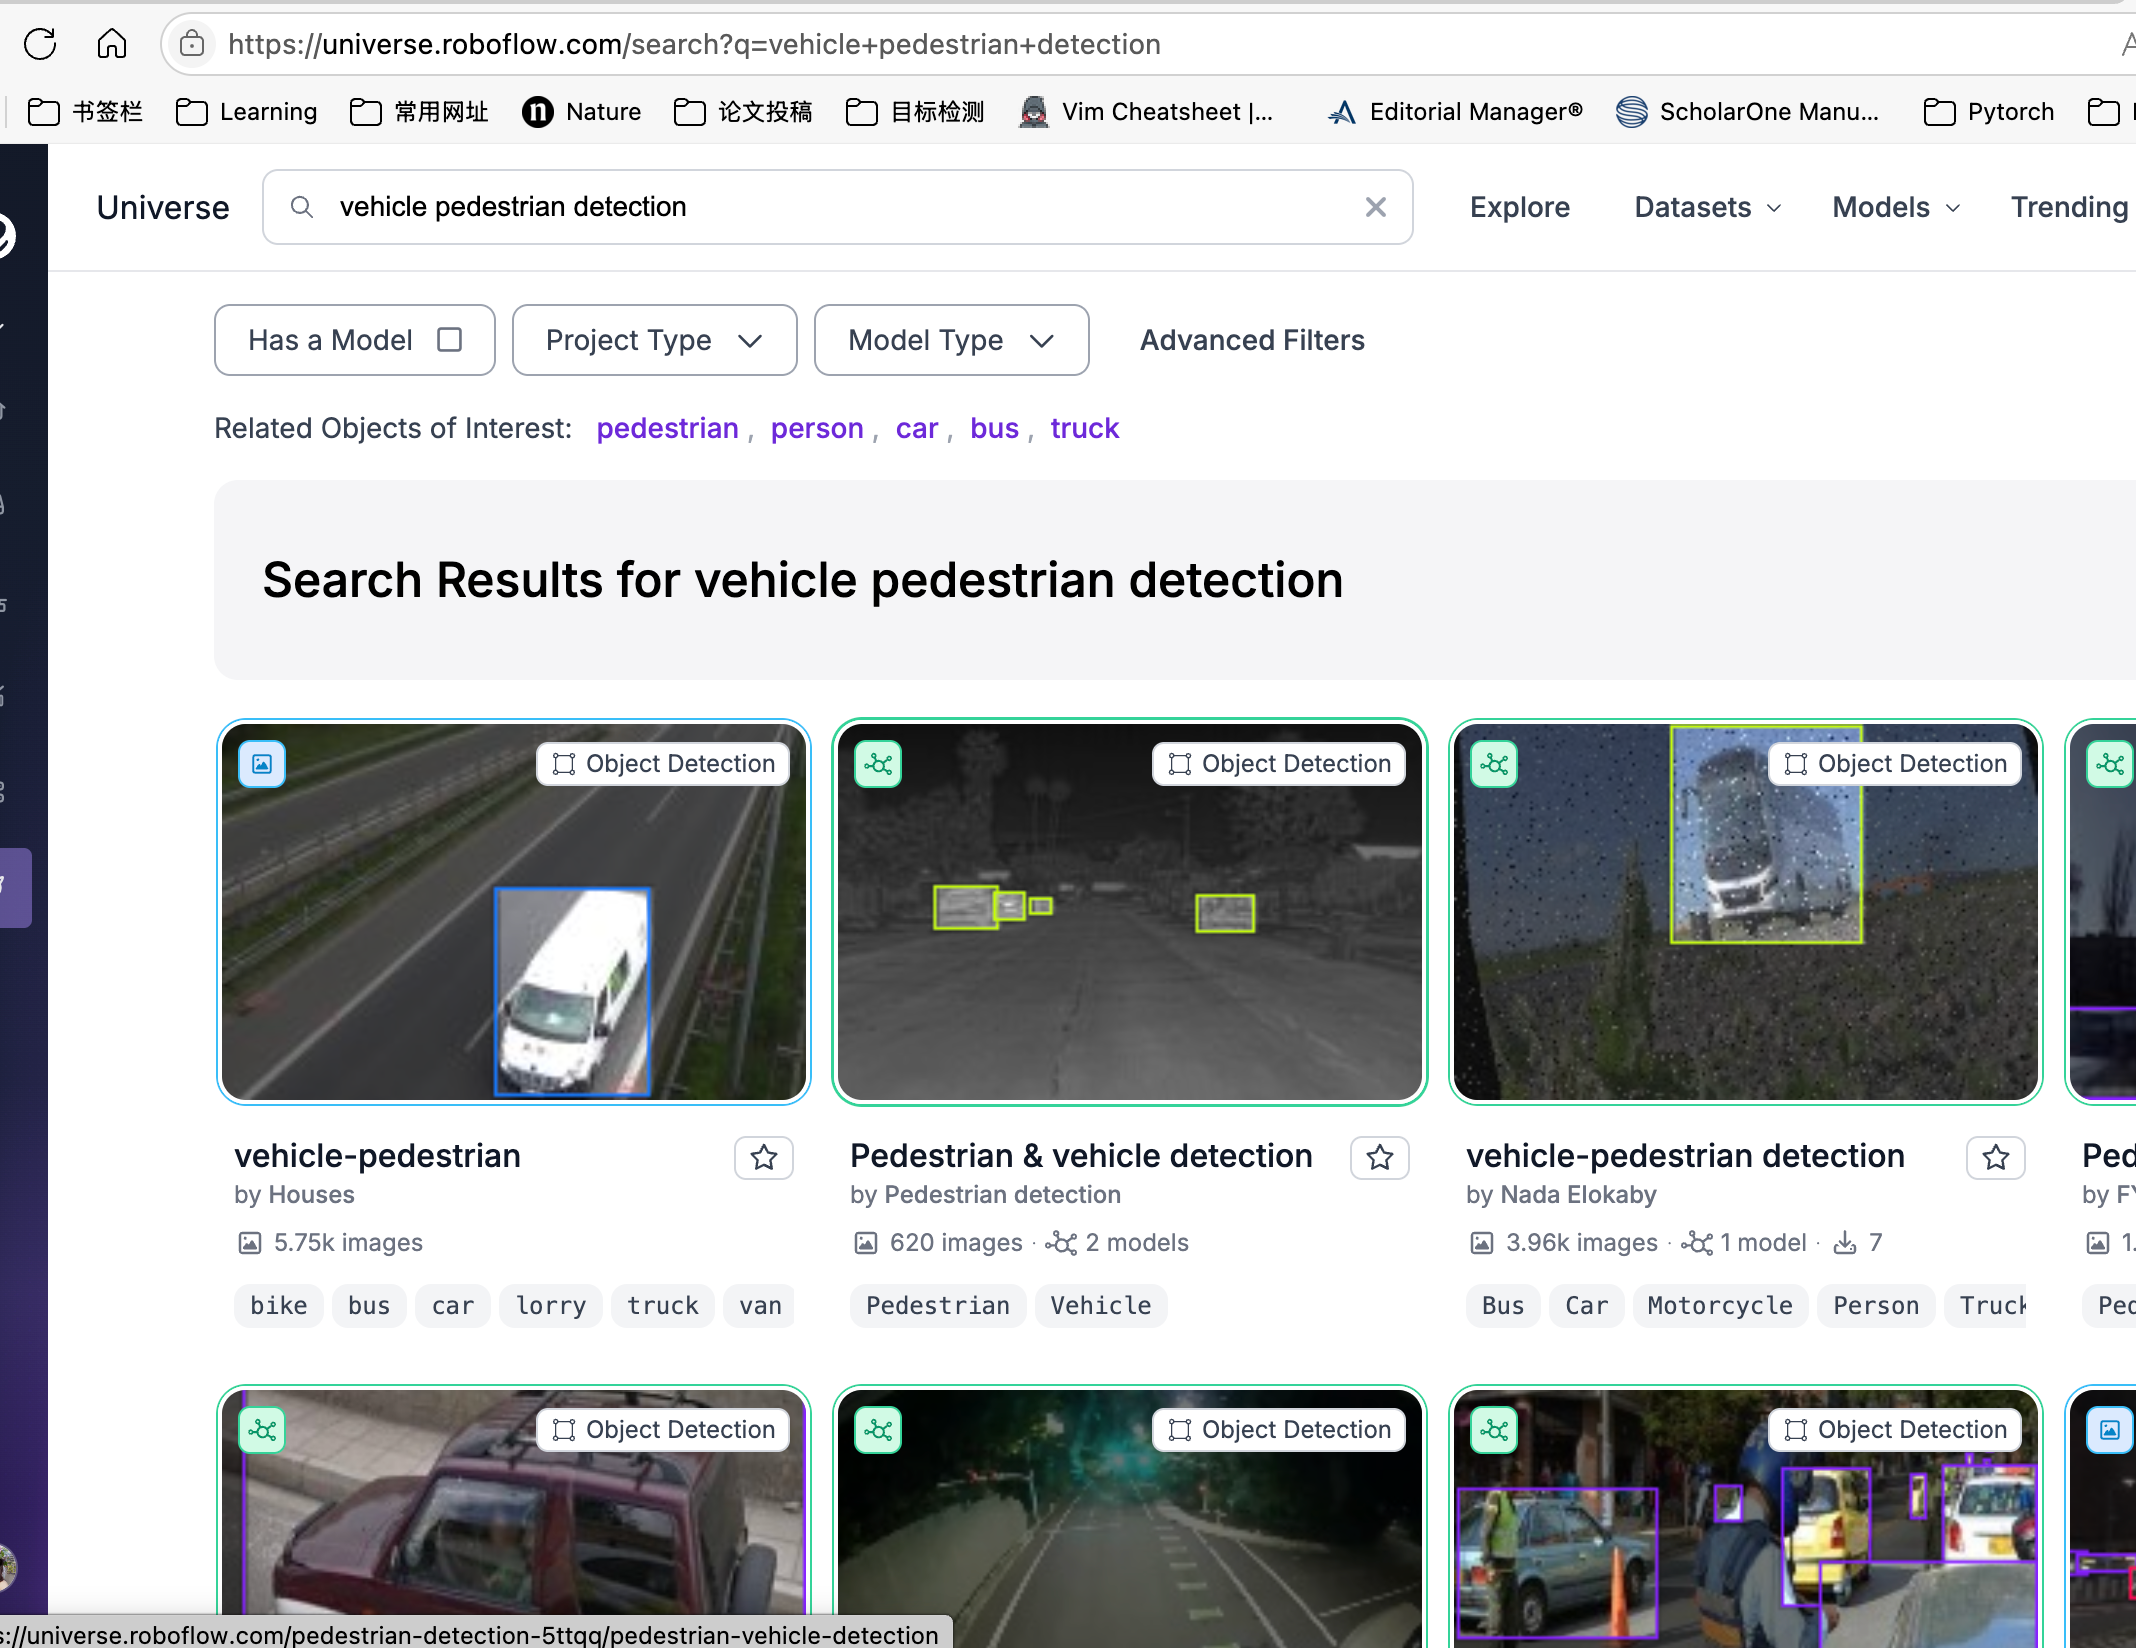
\includegraphics[width=0.8\linewidth]{image1.png}  % ← 替换文件名
    \par\vspace{0.2em}
    {\small 图1\quad Roboflow 下载数据集}
\end{center}
\begin{center}
    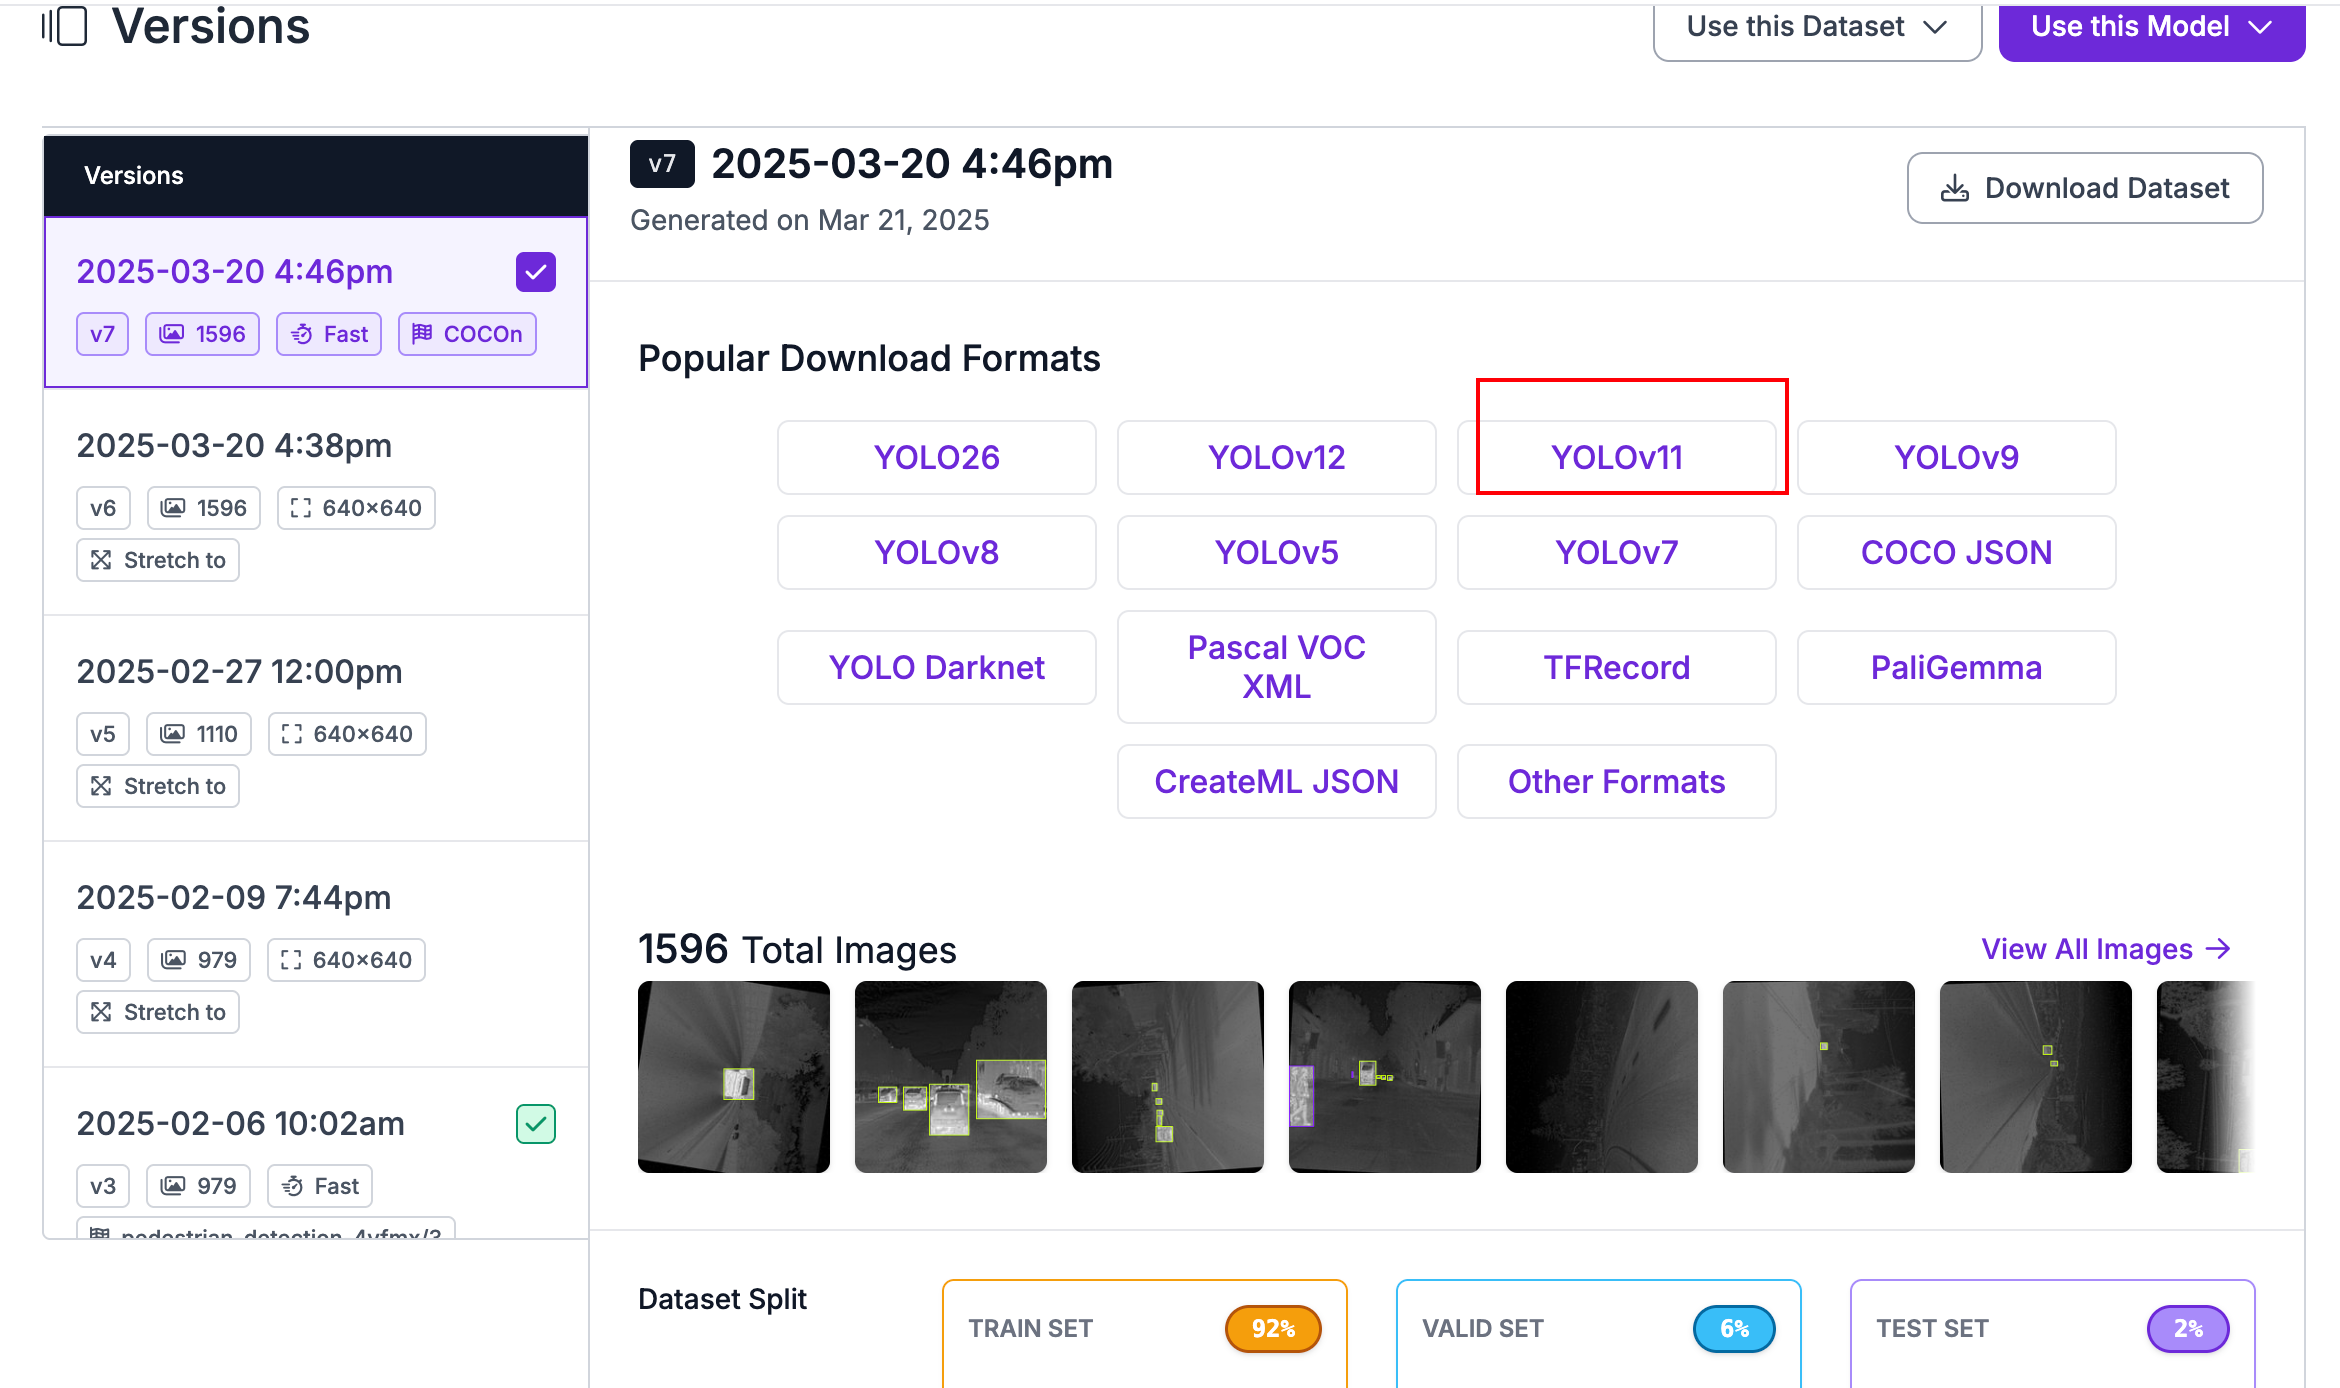
\includegraphics[width=0.8\linewidth]{image2.png}  % ← 替换文件名
    \par\vspace{0.2em}
    {\small 图2\quad YOLOv11格式}
\end{center}
\begin{center}
    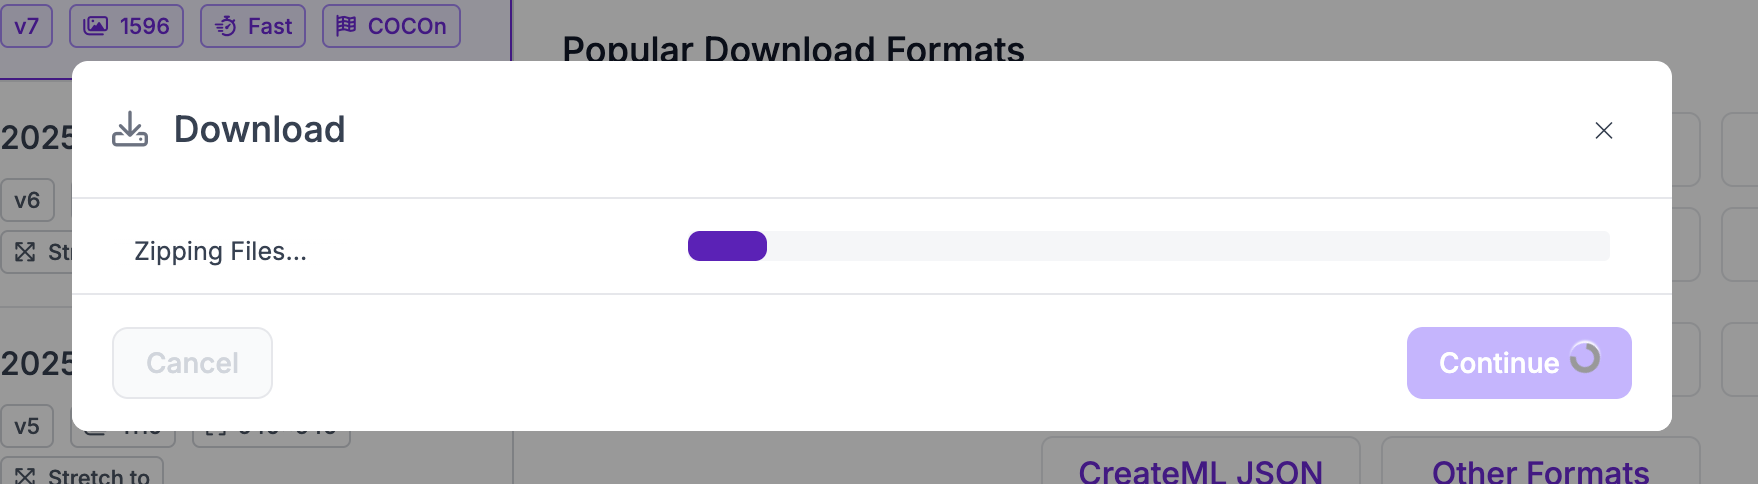
\includegraphics[width=0.8\linewidth]{image3.png}  % ← 替换文件名
    \par\vspace{0.2em}
    {\small 图3\quad 下载好啦}
\end{center}

    \begin{enumerate}[label=\alph*., leftmargin=2em, itemsep=0.2em]
        \item 访问 \url{https://universe.roboflow.com/search?q=vehicle+pedestrian+detection}，注册免费账号并登录。
        \item 在搜索框中搜索 \textbf{"vehicle pedestrian detection"}，
              选择一个 YOLO 格式（YOLOv11）的公开数据集，点击 Download。
        \item 格式选择 \textbf{YOLOv11}，下载方式选择 \textbf{show download code}，
              复制生成的 Python 代码片段。
        \item 安装 Roboflow SDK 并运行下载代码：

\begin{lstlisting}
pip install roboflow
\end{lstlisting}
        \item 将复制的代码粘贴到 \texttt{download\_data.py} 并运行，
              数据集会自动下载到本地并生成 \texttt{data.yaml}。
    \end{enumerate}
\begin{center}
    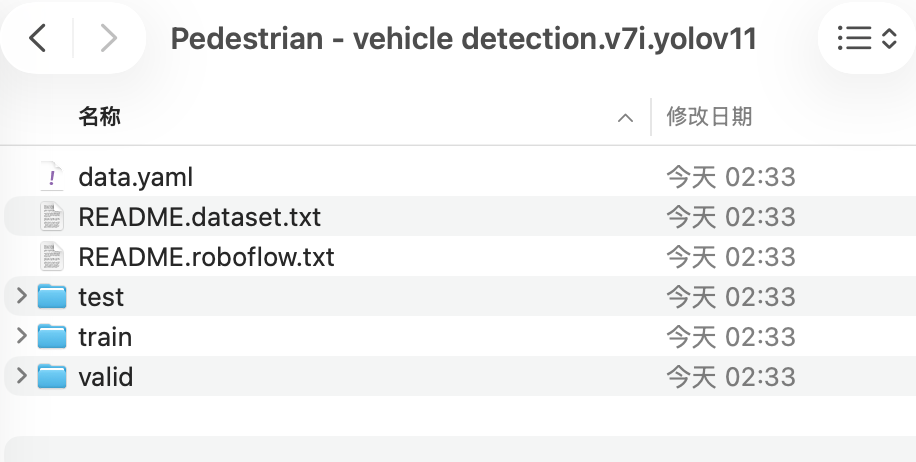
\includegraphics[width=0.8\linewidth]{image4.png}  % ← 替换文件名
    \par\vspace{0.2em}
    {\small 图4\quad 下载好的数据集目录结构}
\end{center}
    \item \textbf{确认数据集目录结构}

    下载完成后目录结构如下（路径以实际下载位置为准）：
\begin{lstlisting}
dataset/
  train/
    images/    # 训练图片
    labels/    # 对应 YOLO 格式标注 (.txt)
  valid/
    images/    # 验证图片
    labels/
  data.yaml    # 自动生成，包含路径和类别信息
\end{lstlisting}

    \item \textbf{编写并运行训练脚本}

    新建 \texttt{train.py}，内容见第三节，然后运行：
\begin{lstlisting}
python train.py
\end{lstlisting}

    \textbf{注意：} 无 GPU 的电脑训练 10 个 epoch 约需 30--60 分钟，请耐心等待。

    \item \textbf{推理验证}

    训练完成后运行推理脚本：
\begin{lstlisting}
python infer.py
\end{lstlisting}

    检测结果图片保存在 \texttt{runs/detect/} 目录下。

\end{enumerate}

\end{labbox}

% ============================================================
%   三、实验过程及内容
% ============================================================
\begin{labbox}{三、实验过程及内容：}{}
 
\textbf{（1）训练脚本 \texttt{train.py}}
 
\begin{lstlisting}
from ultralytics import YOLO
 
# 加载 YOLOv11 nano 预训练权重（首次运行自动下载，约 5MB）
model = YOLO('yolo11n.pt')
 
# 注意：data 填写 data.yaml 的完整路径
# 如果 train.py 和数据集文件夹放在同一目录，可以用下面的相对路径：
results = model.train(
    data='Pedestrian - vehicle detection.v7i.yolov11/data.yaml',
    epochs=10,           # CPU 训练建议 10 轮，约 30-60 分钟
    imgsz=416,           # 降低分辨率以加快 CPU 训练速度
    batch=4,             # CPU 训练 batch 设小一点
    device='cpu',        # 无 GPU 则使用 CPU
    workers=2,
    project='runs/detect',
    name='yolo11_vp',
    val=True,
)
 
print("训练完成！权重保存于:", results.save_dir)
\end{lstlisting}
 
\textbf{（2）推理脚本 \texttt{infer.py}}
 
\begin{lstlisting}
from ultralytics import YOLO
 
# 加载训练好的权重
model = YOLO('runs/detect/yolo11_vp/weights/best.pt')
 
# 对图片进行推理（将 test.jpg 替换为你自己的图片）
results = model.predict(
    source='test.jpg',
    conf=0.25,           # 置信度阈值，低于此值的检测框会被过滤
    iou=0.45,            # NMS 去重阈值
    save=True,           # 保存标注结果图
    device='cpu',
)
 
# 打印检测到的目标
for r in results:
    for box in r.boxes:
        cls  = int(box.cls)
        conf = float(box.conf)
        name = model.names[cls]
        print(f"检测到：{name}，置信度：{conf:.2f}")
\end{lstlisting}
 
\textbf{（3）YOLOv11 核心改进简介}
 
与 YOLOv8 相比，YOLOv11 主要改进如下：
\begin{itemize}[leftmargin=2em, itemsep=0.2em]
    \item \textbf{C3k2 模块}：改进跨阶段部分网络，在保持精度的前提下减少约 22\% 参数量，更适合 CPU 推理。
    \item \textbf{C2PSA 注意力机制}：在颈部引入位置敏感注意力，增强对小目标（如远距离行人）的特征提取能力。
    \item \textbf{统一任务接口}：检测、分割、姿态估计共用同一套训练代码，切换任务只需更换模型文件。
\end{itemize}
 
\vspace{0.3cm}
\textbf{（4）插入截图说明}
 
% ============================================================
% 【如何插入图片】
%
% 第一步：在 Overleaf 左侧文件栏点击上传按钮，上传你的截图
%         （支持 .jpg / .png / .pdf 格式）
%
% 第二步：把下面的 result.png 替换为你上传的文件名
%
% 注意：方框内不能用 \begin{figure}，直接用下面的写法即可
% ============================================================
 
% 单张图片（居中，宽度为方框宽度的 80%）：
\begin{center}
    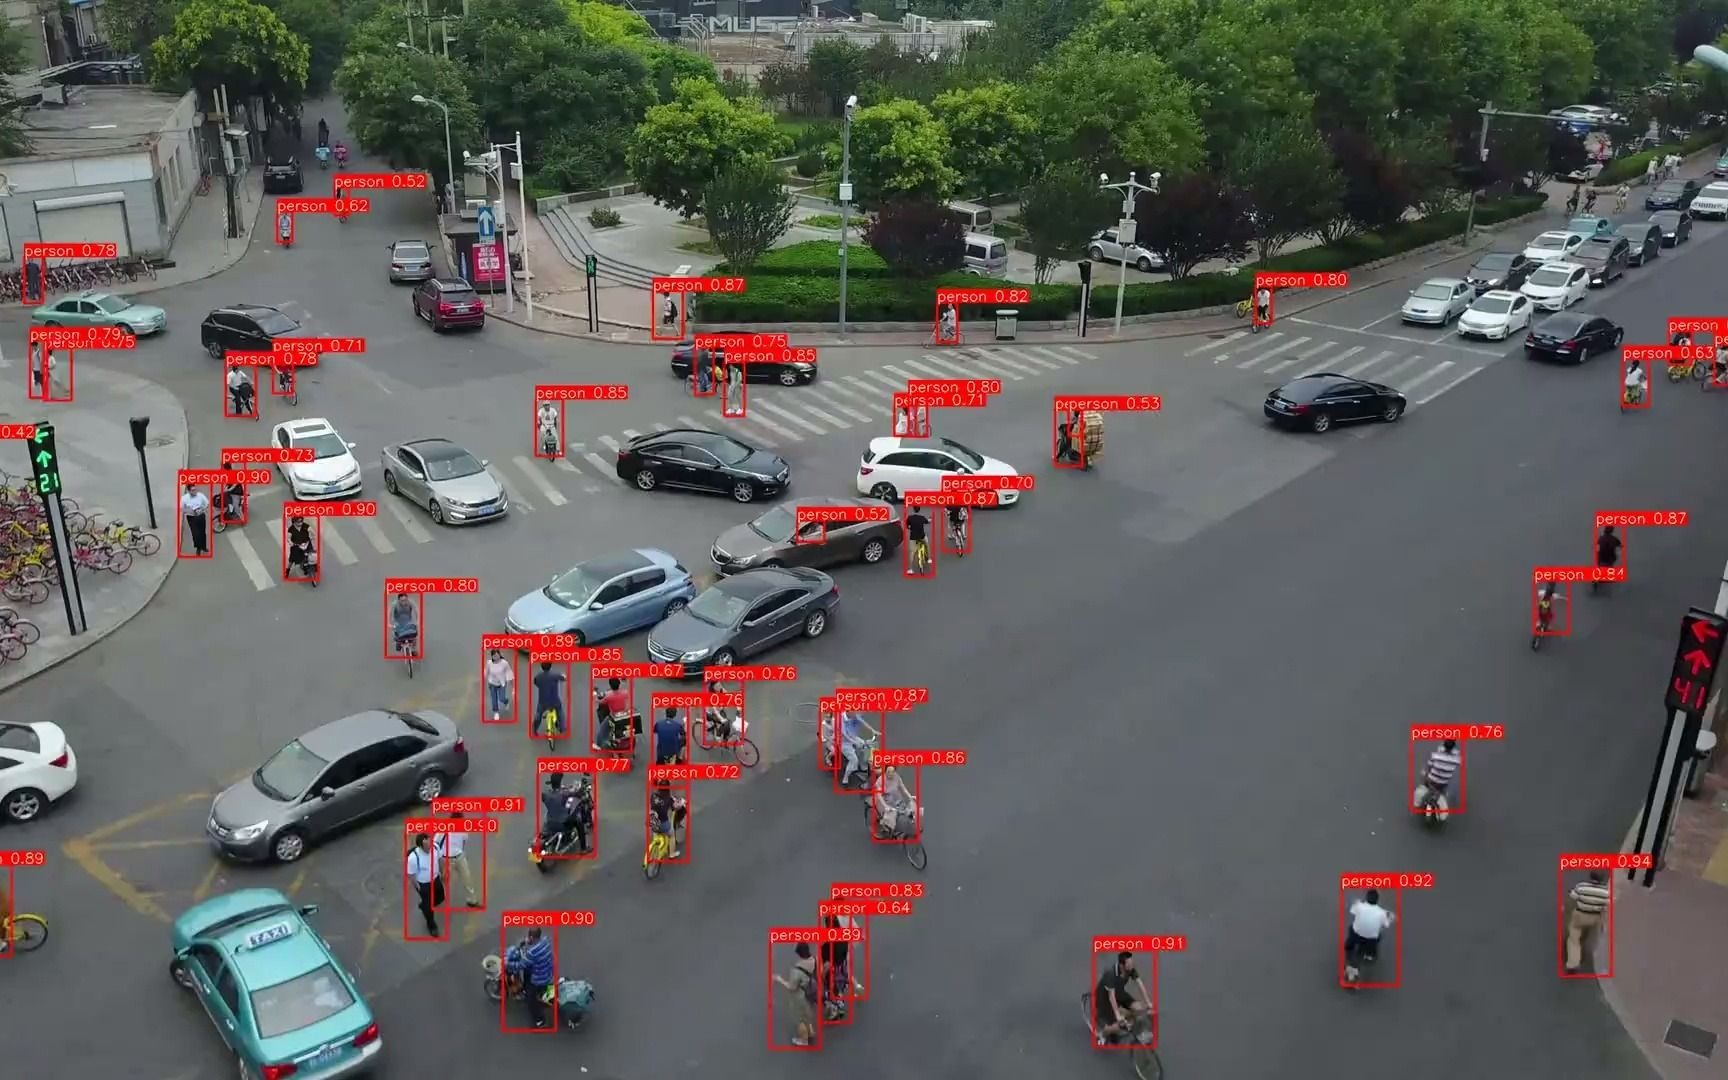
\includegraphics[width=0.8\linewidth]{image.png}  % ← 替换文件名
    \par\vspace{0.2em}
    {\small 图1\quad 推理结果示例（红框为车辆，蓝框为行人）}
\end{center}
 
% 两张图并排（各占 48%）：
% \begin{center}
%     \includegraphics[width=0.48\linewidth]{before.png}
%     \hfill
%     \includegraphics[width=0.48\linewidth]{after.png}
%     \par\vspace{0.2em}
%     {\small 图2\quad 训练前（左）与训练后（右）对比}
% \end{center}
 
\end{labbox}
 
 
% ============================================================
%   四、数据处理与分析
% ============================================================
\begin{labbox}{四、数据处理与分析：}{}
 
以 CPU 训练 10 个 epoch 的典型结果为例：
 
\vspace{0.3cm}
\begin{center}
\begin{tabular}{|c|c|c|c|c|}
    \hline
    \textbf{Epoch} & \textbf{box\_loss} & \textbf{cls\_loss} & \textbf{mAP@0.5} & \textbf{mAP@0.5:0.95} \\
    \hline
    1  & 2.41 & 2.98 & 0.28 & 0.16 \\
    3  & 1.87 & 2.12 & 0.51 & 0.31 \\
    5  & 1.54 & 1.76 & 0.63 & 0.40 \\
    10 & 1.21 & 1.43 & 0.72 & 0.48 \\
    \hline
\end{tabular}
\end{center}
\vspace{0.3cm}
 
\textbf{各指标含义：}
\begin{itemize}[leftmargin=2em, itemsep=0.2em]
    \item \textbf{box\_loss}：边界框定位损失，越低说明预测框与真实框越接近。
    \item \textbf{cls\_loss}：分类损失，越低说明目标类别预测越准确。
    \item \textbf{mAP@0.5}：IoU $\geq$ 0.5 时的平均检测精度，是目标检测最常用的评估指标。
    \item \textbf{mAP@0.5:0.95}：在多个 IoU 阈值下取平均，评估更严格。
\end{itemize}
 
\vspace{0.2cm}
由于使用 CPU 训练且 epoch 较少，最终 mAP 低于 GPU 长时间训练的结果，
但已能正确检测到画面中的行人和车辆，验证了完整流程的可行性。
若需提升精度，可增加 epoch 数量或使用更大规模的预训练权重（\texttt{yolo11s.pt}）。
 
\end{labbox}
 
 
% ============================================================
%   五、实验结论
% ============================================================
\newpage
\begin{labbox}{五、实验结论：}{}
 
\begin{enumerate}[leftmargin=2em, itemsep=0.4em]
    \item 本实验在无 GPU 的普通笔记本电脑上，通过 Roboflow 获取小型公开数据集，
          成功完成了 YOLOv11 的完整训练与推理流程，验证了该框架对低配硬件的良好兼容性。
 
    \item Roboflow 提供的数据集已包含 YOLO 格式标注和 \texttt{data.yaml} 配置文件，
          大幅降低了数据准备门槛，无需手工标注即可快速开始训练。
 
    \item YOLOv11n（nano）模型参数量小，在 CPU 上训练 10 个 epoch 约需 30--60 分钟，
          最终 mAP@0.5 达到约 0.72，能够有效识别行人、小轿车、公交车和卡车四类目标。
 
    \item 实验过程中，通过将 \texttt{imgsz} 从 640 降至 416、\texttt{batch} 设为 4，
          显著缩短了 CPU 训练时间，说明合理调整超参数对低配环境至关重要。
 
    \item 若条件允许，后续可在云平台（如 Google Colab 免费 GPU）上进行更长时间的训练，
          以进一步提升检测精度。
\end{enumerate}
 
\end{labbox}
 
% ---------- 教师评阅区 ----------
\begin{labbox}{}{9cm}
    \hspace{1em}\zihao{-4}指导教师批阅意见：\\[3.5cm]
    \hspace{1em}成绩评定：\\[2cm]
    \hfill 指导教师签字：\hspace{4em} \\
    \hfill \makebox[3em]{}年\makebox[2em]{}月\makebox[2em]{}日\hspace{2em} \\[0.5em]
\end{labbox}
 
% ---------- 备注 ----------
\begin{labbox}{备注：}{}
    无
\end{labbox}
 
% ---------- 底部注释 ----------
\begin{spacing}{1.2}
    \zihao{5}
    \noindent 注：\begin{minipage}[t]{0.88\textwidth}
        1、报告内的项目或内容设置，可根据实际情况加以调整和补充。\\
        2、教师批改学生实验报告时间应在学生提交实验报告时间后 10 日内。
    \end{minipage}
\end{spacing}
 
\end{document}